\documentclass[12pt,a4paper]{report}
\usepackage{dissertation}

\makenoidxglossaries
%Acronyms

\newacronym{cpo}{cpo}{complete partial order}

\newacronym{era}{ERA}{Exact Real Arithmetic}

\newacronym{ode}{ODE}{Ordinary Differential Equation}

\newacronym{ivp}{IVP}{Initial Value Problem}



%Glossary

\newglossaryentry{real}
{
    name={real number/real},
    description={An element of $\R$, which can be defined as the completion of $\Q$ under Cauchy limits}
}

\newglossaryentry{computable_real}
{
    name={computable real number/computable real},
    description={A computational object that denotes a real number}
}

\newglossaryentry{exact_real_arithmetic}
{
    name={exact real arithmetic},
    description={Arithmetic on computable reals}
}

\newglossaryentry{cr_representation}
{
    name={computable real representation strategy/computable real representation},
    description={A mathematical formalization of the concept of computable real (\textit{e.g.} nested intervals representation, modulus of convergence representation)}
}

\newglossaryentry{cr_implementation}
{
    name={computable real implementation},
    description={A concrete implementation of a computable real representation strategy, usually offering functionality like arithmetic, comparison, etc (\textit{e.g.} the packages analyzed in this dissertation)}
}

\newglossaryentry{cr_approx}
{
    name={computable real approximation},
    description={A real value, or range of real values, produced by a computable real number to approximate the real number it denotes. Usually restricted to $\Q$ or some subset of $\Q$}
}

\newglossaryentry{comp_real}
{
    name={\textit{CompReal}},
    description={A Haskell typeclass defined in this dissertation that abstractly encapsulates the concept and functionality of a computable real}
}

\newglossaryentry{comp_real_instance}
{
    name={\textit{CompReal} instance},
    description={A computable real implementation that instantiates the \textit{CompReal} typeclass. All 5 analyzed packages had a \textit{CompReal} instance written for them}
}
\glsaddall

\makeindex

\logo{EE}{School of Engineering}{}
\logoB{EE}{School of Engineering}{}


\author{Tiago Miguel Moreira Bacelar Pereira}

\titleA{Simulation of Hybrid Systems}
\titleB{via Exact Real Arithmetic}
%\titleC{Title Title Title Title}

\masters{Master’s Dissertation in Informatics Engineering}
%\area{Area of specialization}
\supervisor{Renato Neves}

\bibpunct[,]{(}{)}{;}{a}{,}{,}
\begin{document}
\setlength{\parindent}{0em}

%-- Covers
\input{covers/Covers}

%-- Document setup
\newgeometry{right=25mm, left=25mm, top=25mm, bottom=25mm}
\pagenumbering{roman}

\setlength{\parskip}{0pt}
\setlength{\parindent}{1.5em}

%-- Preamble
\chapter*{Copyright and Terms of Use for Third Party Work}
\setlength{\parskip}{1em}
\noindent
This dissertation reports on academic work that can be used by third parties as long as the internationally accepted standards and good practices are respected concerning copyright and related rights.

\noindent
This work can thereafter be used under the terms established in the license below.

\noindent
Readers needing authorization conditions not provided for in the indicated licensing should contact the author through the RepositóriUM of the University of Minho.

\section*{License granted to users of this work:}

\noindent

\includegraphics[]{images/CCBY.png}
\\
\textbf{CC BY}
\\
\url{https://creativecommons.org/licenses/by/4.0/}


\setlength{\parskip}{0em}
\chapter*{Acknowledgements}
\setlength{\parskip}{1em}

This work is financed by National Funds through FCT - Fundação para a Ciência e a Tecnologia, I.P. (Portuguese Foundation for Science and Technology) within project IBEX, with reference 10.54499/PTDC/CCI-COM/4280/2021, and within project Banksy, with reference COMPETE2030-FEDER-00892000.

I want to thank my supervisor, Renato Neves, for his rigor with my work and his patience with me. This dissertation wouldn't be possible without your guidance.

I also want to thank my friends, who I'm so lucky to always have by my side. To everyone who stayed with me throughout this journey: I couldn't have done this without your kindness.

And lastly, to my family, who gave me the blinding light of their dreams. The composure you taught me will follow me all my life. I couldn't face this challenge without your example.


Though the path is long and winding, only by walking it can you reach new horizons. So do not fear the rain, for no matter how bad it gets, you will be warm again. Do not fear your heart, for as much as it hurts it is wonderful to feel. And above all else, do not fear your scars, for, despite everything, it's still you.

\setlength{\parskip}{0em}
\input{preamble/StatementofIntegrity}
\chapter*{Abstract}

%CONTEXT
%hybrid systems
%use floating point arithmetic, which causes errors
%thats bad for some applications
%STATEMENT
%lets use exact real arithmetic
%STATE OF THE ART
%drawing from previous research on computable reals, backed by domain theory, as well as a monadic formalization of hybridness
%GOALS
%implement a hybrid simulator and assess its performance
%METHODS
%in Haskell
%using ERA libraries
%benchmarking
%FINDINGS
%ERA overall is much slower than floating'point, as expected
%some strategies are better than others
%IMPLICATIONS
%the practical tool, Jaguar (namedrop sooner) is pretty cool and can be used for stuff
%future ERA libraries can also learn from these results

Like most programs, simulations of hybrid systems mostly use floating-point arithmetic, which can introduce errors and lead to false conclusions, especially in sensitive and critical systems. This dissertation aims to fix this problem through the use of exact real arithmetic in hybrid programs. Drawing from previous research on computable real numbers backed by domain theory, as well as a monadic formalization of hybridness, a new hybrid simulator Jaguar is developed in Haskell using preexisting exact real arithmetic libraries. The greatest challenges in development are the semidecidability of comparison between computable reals and the implementation of a differential equation solver. As expected, the final product is overall slower than equivalent programs using floating-point; but there are interesting performance differences between various exact real arithmetic libraries due to their different strategies and characteristics, as explored in the benchmarking. These results are doubtlessly of interest from the perspective of designing new performant exact real arithmetic libraries, and Jaguar as a standalone tool has applications in (small) physical simulations, formal verification and more.

\paragraph{Keywords} exact real arithmetic, hybrid systems, Jaguar, computable real numbers

\cleardoublepage

\chapter*{Resumo}

Tal como a maioria dos programas, as simulações de sistemas híbridos utilizam maioritariamente aritmética de vírgula flutuante, o que pode introduzir erros e levar a conclusões incorretas, especialmente em sistemas críticos ou sensíveis. Esta dissertação procura resolver este problema através da utilização de aritmética real exata em programas híbridos. Com base em investigação existente sobre números reais computáveis baseada em teoria de domínios, bem como numa formalização monádica da natureza híbrida destes sistemas, foi desenvolvido um novo simulador híbrido em Haskell chamado Jaguar, recorrendo a bibliotecas pré-existentes de aritmética real exata. Os maiores desafios durante o desenvolvimento foram a semidecidibilidade da comparação entre números reais computáveis e a implementação de um solver de equações diferenciais. Como seria de esperar, o produto final é, de um modo geral, mais lento do que programas equivalentes que usam aritmética de vírgula flutuante. No entanto, as bibliotecas de aritmética real exata apresentam entre si diferenças de desempenho, resultantes das suas diferentes estratégias e características, tal como demonstrado no benchmarking. Estes resultados são relevantes para o desenvolvimento de futuras bibliotecas de aritmética real exata de alto desempenho. Além disso, o Jaguar, enquanto ferramenta autónoma, tem aplicações em simulações físicas de pequena escala, verificação formal e outras áreas.

\paragraph{Palavras-chave} aritmética real exata, sistemas híbridos, Jaguar, números reais computáveis

\cleardoublepage


\phantomsection
\tableofcontents

\cleardoublepage
\listoffigures

% List of tables
\renewcommand*{\listtablename}{List of Tables}
\listoftables
\clearpage


% Acronyms
\printnoidxglossary[type=\acronymtype, title={Acronyms}, sort=def, nonumberlist]

% Glossary
\printnoidxglossary[title={Glossary}, sort=def, nonumberlist]

\cleardoublepage
\pagenumbering{arabic}

%-- Dissertation 
%\part{Introductory material}

\bibliographystyle{unsrtnat}
\setcitestyle{square,numbers}

\theoremstyle{definition}
\newtheorem{exmp}{Example}[section]

\chapter{Introduction}
\label{chap:intro}

\section{Context and Motivation}

Hybrid systems are commonly defined as processes that possess a mix of both continuous evolution, usually modeled through differential equations, and discrete behaviors, such as conditionals, assignments and other instantaneous changes \cite{neves18}. This model proves invaluable, specifically when simulating the interaction of physical, continuous processes with software-controlled systems, such as cruise controllers and pacemakers. The resulting programs are known as hybrid programs.

Taking the example of a cruise controller, we can write a simple program that checks the velocity of a vehicle every second and either accelerates or brakes, eventually hovering around the target velocity. The following program was implemented in Lince \cite{goncharov2020}, an imperative hybrid programming language and simulator:

%todo: meter o case study (ACC leader) aqui em vez deste CC?
\begin{lstlisting}[caption=Example of a hybrid program]
v:=4;
while true do {
    if v<=10 then v'=1 for 1; else v'=-1 for 1;
}
\end{lstlisting}

\begin{figure}
    \centering
    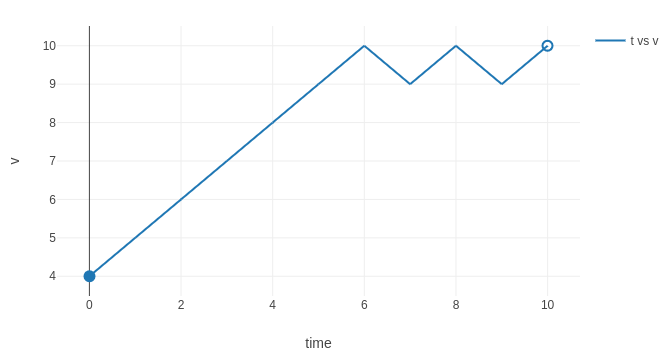
\includegraphics[width=0.75\linewidth]{images/cc_plot.png}
    \caption{Plot of the velocity over time in the cruise control program}
    \label{fig:cc_plot}
\end{figure}

The program starts by assigning the value 4 to variable v. The statement inside the while loop will either accelerate or break, depending on the current velocity, by setting the derivative of $v$, $v'$, to 1 or -1 during 1 second. The while loop indicates that this behavior repeats indefinitely. This appears to be a non-terminating program, because of the infinite while loop, but the evaluation at any specific time will only go through a finite number of iterations of the loop. A plot of the simulated velocity over time can be found in \autoref{fig:cc_plot}.

Despite simple, this example illustrates the basic concepts of a hybrid program, namely the presence of both classical assignment, control structures, etc. as well as differential, continuous constructs and their relation to time.

Among the many difficulties of this paradigm, one of the greatest is the often overlooked matter of precision and error. When developing proper methods of simulation, the standard way to represent numbers is floating point arithmetic, which treats values as a mantissa and an exponent. This system can be, and sometimes is, used to represent numbers with an arbitrary precision, but is usually implemented with a finite precision by limiting the size of the mantissa and exponent. This is enough for most applications, but especially in chaotic systems, where errors compound, the precision limit can be easily exhausted, and any value outputted by the program will stray further and further from the actual value of the calculation. Lince itself uses standard floating point numbers with 64 bits of precision, known as double in most programming languages, which makes it prone to errors when the values get too close to zero. Take the following program as an example:

%   x:=2;
%   x'=1-x for 35;
%   x'=x-1 for 35;
\begin{lstlisting}[caption=Hybrid program showcasing insufficient precision]
x:=1;
x'=-x for 80;
x'= x for 80;
\end{lstlisting}

\begin{figure}
    \centering
    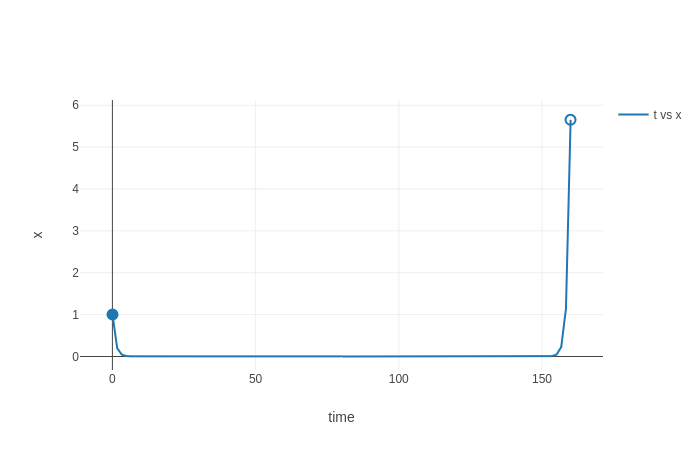
\includegraphics[width=0.75\linewidth]{images/exp_plot.png}
    \caption{Plot of $x$ over time in the exponential program}
    \label{fig:exp-plot}
\end{figure}

\autoref{fig:exp-plot} is a plot of the simulation of variable $x$ over time. Variable $x$ was expected to go from 1 to a very small number at time $t=80$ following a negative exponential ($e^{-t}$), and then follow a positive exponential ($e^t$) afterwards and bounce back to 1 at time $t=160$. But the Lince simulator shows the final value of $x$ as 5.653719, which is clearly an error. This error grows even larger if we replace 80 with even larger values.

Using an arbitrary number of digits to represent values, together with ratio representations (numerator and denominator), allows for the exact representation of all rational numbers, but still leaves open the problem of irrational numbers, which are common when simulating physical systems (when using trigonometric functions, for instance, or with the previous exponential example). Unlike their rational counterparts, it would take an infinite number of digits to represent an irrational number using a regular digit representation. This problem therefore calls for alternative solutions.


\section{Goals}

The goal of the project is the simulation of hybrid systems through the use of exact real arithmetic. More specifically, the project consists of implementing a hybrid system simulator based on preexisting libraries for exact real arithmetic. Simulator performance is expected to be worse than simulators using floating point arithmetic such as the aforementioned tool Lince \cite{goncharov2020}, but should be perfectly faithful to the real system simulated.

The hybrid systems' specification language will be based on a while language with specific constructs to describe the behavior of physical processes. This choice is due to the simplicity and power of the language, which furthermore has a well-established operational semantics that can be used as a basis for implementation. The simulator will be implemented in the Haskell programming language due to its lazy paradigm and use of higher-order functions, which are particularly useful in the context of exact real arithmetic.

\section{Overview}

As a theoretic work, this thesis is mostly about compiling and systematizing already existing research from the fields of exact real arithmetic and hybrid systems. There is a wealth of research on exact real arithmetic, mostly on its more theoretical aspects (a good summary of which can be found in \cite{geuvers07}). This thesis looks at multiple representation strategies from a more practical angle, how they are related, and their unique advantages and disadvantages. As for hybridness, since the topic is already well studied and systematized in the literature, it is presented here in a mostly non-transformative manner, and limited only to the more relevant concepts for the practical implementation of the simulator.

Original theoretical contributions are mostly limited to what was needed to implement the hybrid simulator. Due to fundamental limitations of exact real arithmetic, the simulator can't be implemented directly, instead requiring alternatives and workarounds to combine the two technologies. The main limitation to overcome is the undecidability of comparison in exact real arithmetic, which isn't guaranteed to eventually halt if evaluated totally. The workaround presented in this thesis (\autoref{sec:undecidability}) is instead using partial comparison, up to some accuracy. This workaround forces the operations on hybrid structures to be rewritten as parametrized operations, taking as a parameter the accuracy of the partial comparisons.

The other big challenge to overcome is implementing a differential equation solver that produces a single exact real value as its output. Numerical methods for solving differential equations, like the famous Runge-Kutta\todo{ref}, only generate approximations of the wanted result; and despite being able to reach arbitrarily good approximations (by lowering the step size, for instance), they don't provide strict error bounds for their results, which makes it impossible to convert into an arbitrary-precision real value. The solution presented in this thesis (\autoref{sec:solver}) starts by transforming the equations into a system of polynomial equations. The system is then solved using the equations' Taylor series, obtained with forward automatic differentiation, and a fixed step size to calculate the approximations (which can be arbitrarily improved by taking more and more elements of the Taylor series). The error bound of the results is calculated using the results of the paper "Explicit A-Priori error bounds and Adaptive error control for approximation of nonlinear initial value differential systems" \cite{WARNE20061695}.

On the practical side, this thesis is a comprehensive exposition of the inner workings and functionality of the developed simulator, Jaguar. Beyond the features already discussed, Jaguar supports using all the analyzed exact real arithmetic libraries for its computations (as well as double-precision floating-point numbers as well), and provides an easy base for implementing additional numeric types in the future. Jaguar is also highly configurable, allowing users to choose the parameters of both the simulation and the queries. It also comes with a built-in visualizer using a plotting library, Chart \cite{Chart}.

Though some efforts were made to formalize the new language (see \cref{sec:semantics} for the formalized operational semantics), a lot more could be done in this area, with the ultimate goal being linking the operational and denotational semantics of the language and using the latter to prove its correction.

\section{Document Structure}

After this introduction, \autoref{chap:state_art} gathers the technical background relevant for this project. It first delves into an exploration of existing formalizations and techniques for representing exact real numbers (\autoref{sec:theory}). A study of several open-source libraries follows in \autoref{sec:practice}, where the underlying approaches are compared and critiqued. Then, \autoref{sec:hybrid} lays out the theory behind hybrid systems and presents the underlying challenges of their simulation.

\autoref{chap:implementation} discusses the implementation of the simulator (architecture overview in \autoref{sec:architecture}, followed by the parser in \autoref{sec:parser}, interpreter in \autoref{sec:interpreter}, solver in \autoref{sec:solver} and visualizer in \autoref{sec:visualizer}), and exposes the challenges found along the way and their respective solutions, along with other notable implementation details.

In \autoref{chap:results} the performance of the simulator is discussed, and benchmarking results are presented.

Finally, \autoref{chap:conclusion} talks about the general future direction of this research and lists some next steps towards it.

Throughout this thesis, the reader is assumed to be knowledgeable about partial orders, limits, derivatives, Taylor and Maclaurin series, and monads.\todo{refs}

Functors will be represented with an upper-case sans-serif letter (e.g. $\functor{M}$). If the functor generalizes to a monad, this monad is represented by the same letter in bold font weight. The set of natural numbers is represented with $\N$ and is understood to consist of all non-negative integers ($0 \in \N$). $\R_0^+$ represents the set of non-negative reals. $\overline{\R_0^+}$ denotes the extended non-negative reals (i.e. $\R_0^+$ extended with the infinity value \infty). $[0,\R_0^+)$ is the set of all intervals of the form $[0,d), d \in \R_0^+$ (which includes \emptyset, falling from $d=0$). Finally, $[0,\overline{\R_0^+}\rrparenthesis$ denotes the set of all intervals of form $[0,d], d \in \R_0^+$ or form $[0,d), d \in \overline{\R_0^+}$.


%todo: indice de abreviaturas? so far we got:
% IVP, ODE
\chapter{State of the Art}
\label{chap:state_art}

\section{The Theory of Exact Real Arithmetic}
\label{sec:theory}

There is a lot of established theory on exact real numbers, a good overview of which can be found in \cite{geuvers07}. This section presents the basic concept behind a great deal of real number representations, namely infinite sequences of approximations, and explains the mathematical motivations behind it (\autoref{sec:cauchy}). Domain theory is discussed as both a motivation and formalization of the use of intervals as approximations in \autoref{sec:domain}, and the concept of modulus of convergence is presented in \autoref{sec:modulus}. \autoref{precision_accuracy} presents the formal definitions of precision and accuracy from numerical analysis and how they are used in the context of exact real arithmetic. Lastly, \autoref{theory_summary} summarizes the whole section and lists some limitations common to all representation strategies.


\subsection{Cauchy Sequences}
\label{sec:cauchy}

There are multiple formal definitions of real numbers, but the most used definition for exact real number representation is based on Cauchy sequences. Concisely: the set of real numbers $\R$ is the smallest set that contains the rationals and is closed under limits of Cauchy sequences. So a simple and straightforward way to represent a real number is simply as a sequence of rationals. Of use to us, because the rational numbers are dense, this means that any real number can be approximated by a Cauchy sequence of rationals, or indeed any dense subset of the rationals, such as the dyadic numbers (numbers of the form $a/2^p$, with $a,p \in \Z$).

A Cauchy sequence is defined as a sequence whose terms get arbitrarily close to each other, essentially converging on a single number. More formally, $\{a_i\}_{i \in \N}$ is a Cauchy sequence if
\begin{equation}
\label{eq:cauchy}
\forall \epsilon>0, \exists i: \forall j>i, |a_i - a_j| < \epsilon
\end{equation}

This formalization, however, poses a problem: even if a sequence is known to be Cauchy, it is impossible to know which number it is converging into by looking only at a finite number of its terms. For example, the following sequence represents the number 2:

\begin{equation}
  \begin{cases} 
    a_i = 0 & \text{if } i < 1000000 \\
    a_i = 2 & \text{if } i \geq 1000000 \\
  \end{cases}
\end{equation}

In the worst-case scenario, the sequence may not even be Cauchy and not converge. A direct implementation of this concept, also known as the plain or naive Cauchy representation, is therefore insufficient, since it makes no guarantees about the represented real value at any step. 

While insufficient \textit{per se}, Cauchy sequences can still be used as a basis for more sophisticated representation methods. The next sections offer improvements to this basic idea.


\subsection{Domain theory and Interval Arithmetic}
\label{sec:domain}

Domain theory \cite{winskel93} deals with sets equipped with a complete partial order (cpo, here represented as $\sqsubseteq$), called domains, where this order measures the information content of each element of the domain. Each element of a domain can be thought of as a (partial) result of a computation, and one element is greater than another if it extends its information content in a consistent way. Like any partial order, cpos must be reflexive, transitive and antisymmetric. Additionally, every directed chain of the domain (that is, a chain of elements where each element is greater than the previous), must have a least upper bound in the domain. Informally, there is an element of the domain that summarizes all information of any non-contradicting chain of the domain. This property is called completeness.

For example, take the kleenians ($K_3 = \{T, F, U\}$), the 3 possible valuations of a proposition in Kleene's three-valued logic, first introduced in \cite{Kleene_1938}. This domain is of special interest to this dissertation since it will form the basis for the evaluation of propositions in the simulator (\autoref{sec:bool_expr}). The kleenians can be understood as a domain $(K_3,\sqsubseteq)$ where its elements are related as follows: $U \sqsubseteq F$ and $U \sqsubseteq T$ (\autoref{fig:kleenians_dom}). This relation represents the fact that we may have no information about the value of a proposition ($U$), or have mutually exclusive information (the proposition is $T$ or $F$).

\begin{figure}
    \centering
    \includesvg[width=0.75\linewidth]{images/kleenians.svg}
    \caption{Hasse diagram of the domain of the kleenians}
    \label{fig:kleenians_dom}
\end{figure}

Another example of a domain, also of interest later in the dissertation, is the ordering domain, which extends the 3 relative positions obtained from comparing two real numbers ($a < b$ - LT, $a = b$ - EQ - and $a > b$ - GT) into a domain, where each element of the domain represents a possible state of knowledge about the relative position of the two reals, as shown in \autoref{fig:ordering_dom}:

\begin{figure}
    \centering
    \includesvg[width=0.75\linewidth]{images/ordering_dom.svg}
    \caption{Hasse diagram of the ordering domain}
    \label{fig:ordering_dom}
\end{figure}

Domain theory is the basis of denotational semantics of programming languages, since it models the idea of computational information. A computation can be thought of as a continuous function, that is, a monotonic function such that, for any subset $X$ of the domain:

\begin{equation}
\bigsqcup_{\substack{x \in X}} f(x) = f(\bigsqcup_{\substack{x \in X}} x)
\end{equation}

where $\bigsqcup$ denotes the least upper bound. Another recurring concept in domain theory is the bottom element $\bot$ of a domain $D$, which, when it exists, is defined as the least element of $D$ ($\forall x \in D, \bot \sqsubseteq x$ - that is, $\bot$ is the only minimal element of $D$) and denotes no information or a never-ending computation. In the previous examples, both domains have a bottom element.

To represent real numbers, it is interesting to work specifically with the domain of closed real intervals, the reason for which will shortly become apparent. We define the domain $(I,\sqsubseteq)$ as:

\begin{equation}
[a,b] \sqsubseteq [c,d] \iff [a,b] \supseteq [c,d]
\end{equation}

from which we can derive

\begin{equation}
\bigsqcup_{\substack{[a,b] \in X}} [a,b] = \bigcap_{\substack{[a,b] \in X}} [a,b]
\end{equation}

This means that an interval has greater information content than another if it is contained in it. In this domain, a maximal element is an interval with zero length, that is, an interval of the form $[a,a]$, since the only interval contained in it is itself ($[a,a] \supseteq [b,c] \rightarrow [a,a] = [b,c]$, or equiavalently, $[a,a] \sqsubseteq [b,c] \rightarrow [a,a] = [b,c]$, which is the definition of a maximal element in $\sqsubseteq$). $[a,a]$, therefore, denotes exactly the real number $a$. Crucially, because computations correspond to continuous functions on the domain, any computation on a set of converging intervals will approach the result of the computation applied to the denoted real number.

This suggests how a possible implementation might be structured \cite{BAUER2009251}: a real number should be represented by a sequence of nested rational intervals, so that each interval of the sequence collects all of the information of the previous ones. This way, we have solid theoretical ground to know that an operation to the sequence of intervals will approach the result of the operation of the denoted real number, and that each resulting interval is at least as accurate as the previous ones.

As a small aside, it is important to keep in mind that operating on an interval is, in general, harder than operating simply on its endpoints. While that is the case for monotonic operations on real numbers, such as addition and subtraction (e.g. the sum of two intervals is the interval whose endpoints are the sum of the terms' endpoints), in general it may be necessary to consider the whole interval (when calculating the sine of an interval, for instance). As a result, exact real representations through sequences of nested intervals have a greater computational cost on operations than plain Cauchy sequence representations.


\subsection{Modulus of Convergence}
\label{sec:modulus}

Although nested intervals allow the sequence to bound every approximation's error, note that it does not actually guarantee that any sequence converges on a single real number; it may simply converge on an interval. To ensure the former, we must introduce what is known as a modulus of convergence. The modulus of convergence is defined as follows: for a given Cauchy sequence $\{a_i\}_{i \in \N}$, the modulus of convergence is a function $f:\N \rightarrow \N$ that satisfies the following relation:

\begin{equation}
i \geqslant j > f(n) \implies |a_i - a_j| \leq 2^{-n}
\end{equation}

Informally, for a certain $n$, the modulus of convergence gives us a position on the sequence such that all future terms differ less than $2^{-n}$ from each other, therefore implying that all of these terms have an accuracy of at least $n$. If such a function exists, it is possible to prove that the sequence follows \autoref{eq:cauchy} and therefore converges.

To avoid treating the sequence and its modulus separately, an exact real number representation may enforce that its sequences follow a fixed modulus of convergence $f(n) = n$, to which any arbitrary sequence can be converted by composing with its modulus of convergence: $[c,d]_i = [a,b]_{f(i)}$.

In practice, many representations don't provide a modulus of convergence, since calculating and enforcing it comes with added computational costs, and instead settle for nested intervals. When they do, the only way to evaluate the represented real number up to a certain accuracy is to advance through the sequence until the wanted accuracy is met.

Lastly, note that a Cauchy sequence $\{a_i\}_{i \in \N}$ equipped with a modulus of convergence $f:\N \rightarrow \N$ can be converted into a valid sequence of nested intervals $\{[b,c]_n\}_{i \in \N}$, since the modulated terms of the sequence effectively form an interval of length $2^{-n}$:

$[b,c]_n = [a_{f(n)}-2^{-n-1}, a_{f(n)}+2^{-n-1}]$

This makes nested intervals a sort of intermediate step between the basic Cauchy sequences with no modulus, the least restrictive representation (so nonrestrictive, in fact, that it is insufficient for practical use), and sequences with a modulus, which have the most restrictions. For example, to represent the number 2, a plain Cauchy sequence has literally no restrictions on any finite number of its elements (see the example at the end of \autoref{sec:cauchy}); a sequence of nested intervals forces all its intervals to contain the number 2 (but does not restrict the length of the intervals in any way); and a modulus of convergence sets a maximum interval length that gets cut in half for each new interval.



\subsection{Precision vs Accuracy}
\label{precision_accuracy}

Since these two terms are used interchangeably in day-to-day language, it may be helpful to revisit their formal definition in numerical analysis and how they apply in exact real arithmetic in particular.

Accuracy refers to how close the result of a computation or approximation is to the mathematical true value being computed, measured by the absolute or relative error of the approximation. In this thesis, accuracy is denoted by $n$ \footnote{As implied by the choice of symbol, $n$ is a natural number ($n \in \N$). Although it wouldn't be nonsensical to consider negative accuracies as well (that is, absolute errors greater than $0.5$), in practice, sequence of approximation-type representations are usually limited to natural accuracies for ease of implementation} and is defined logarithmically in terms of the absolute error $\epsilon$:

$n = \lfloor-log_2(\epsilon)-1\rfloor$

This quantity is, not incidentally, the input of the modulus of convergence of a Cauchy sequence. If the accuracy $n$ of a certain result or approximation $\hat{x}$ is known, we can construct an interval of length $2^{-n}$ of all possible values for the computation's true value $x$:

$ \hat{x}-2^{-n-1} \leq x \leq \hat{x}+2^{-n-1} $

For instance, take $50/16=3.125$ as an approximation of pi. This approximation has an error of $\epsilon = |\pi-50/16| = 0.016592...$, from which we derive its accuracy of $n=\lfloor-log_2(0.016592...)-1\rfloor = 4$. This means that in a Cauchy sequence converging to pi that follows a constant modulus of convergence ($f(n)=n$), this approximation could be any of the first five terms. Of course, this example is, in a sense, "backwards", since we used the actual value of pi to calculate the error (and then accuracy) of our approximation. In reality, the reason why we generate approximations is to approach an unknown true value, and so the error has to be inferred from the nature of the operations performed to obtain the approximation. This process of error inference is an important part of numerical analysis, and extremely relevant to us here as well: we want to generate error bounds as tight as possible for the amount of computational resources expended, so as to maximize performance.

%what is precision
Precision, on the other hand, is the resolution of the result's representation, usually given as the number of decimal or binary digits. More formally, \textit{Accuracy and Stability of Numerical Algorithms} \cite{AccNumAlg} defines precision as "the accuracy with which the basic arithmetic operations $+$, $-$ , $*$, $/$ are performed". As an example, take dyadic numbers: for a fixed $p$ and any integer $a$, dyads of the form $a/2^p$ may be said to have a precision of $p$, since operations may cause errors of at most $1/2^{p+1}$ - exactly half of the "hole" between consecutive dyadic numbers\footnote{This is equivalent to how precision is usually discussed in computer science (in the context of floating-point numbers), but considering the alternative definition of accuracy using relative error instead of absolute error. Floating-point is essentially an attempt to minimize the relative error caused by the "holes" between consecutive floating-point numbers, while dyadic numbers attempt to minimize the absolute error}.

%why precision limits accuracy
This example also illustrates how the precision of dyadic numbers (and, indeed, any other arithmetic) interacts with the accuracy of computations: while some computations (like addition and subtraction) can be performed with perfect accuracy (e.g. $1/2^0+2/2^0=3/2^0$), in the worst-case scenario (where the true value of a result is right in the middle of a "hole"; for example, $1/2^0 \div 2/2^0$), accuracy is limited by the precision of the approximation ($n \leq p$), independently of the result.

%why accuracy is more important
While precision is important when discussing the development and inner workings of an algorithm or calculation, end users are usually more interested in a result's accuracy, or, equivalently, on an error bound for the result. Consider the aforementioned example of $50/16=3.125$ as an approximation for pi. If it is interpreted as the dyadic number $50/2^4$, then this approximation has a precision of $p=4$. However, notice that $51/2^4$, $-42/2^4$, or indeed \textit{any} dyadic number with the same denominator also has a precision of $4$, even though they aren't remotely close to pi. Even though $50/2^4$ is the \textit{best} approximation with precision $4$, it is far from the only one. That being said, it is true that \textit{because} it is the best approximation with precision $4$, $50/2^4$ will necessarily have an accuracy of (at least) $4$.

It is worth mentioning that, in the context of arbitrary-precision (and arbitrary-accuracy) arithmetic, it makes no sense to talk about the precision or accuracy of a number, since each number can be approximated to arbitrarily high accuracy. Precision and accuracy are only relevant when discussing the number's approximations.


\subsection{Summary}
\label{theory_summary}

%To summarize, all presented methods of exact real representation rely on sequences of increasingly accurate approximations. If the approximations are plain numbers, it is a Cauchy sequence. If the representation uses a sequence of shrinking intervals, it is a nested intervals representation, that allows the sequence to keep track of its accuracy at each step. Finally, if the sequence contains a modulus of convergence, or follows a fixed modulus, it is able to make guarantees about the speed of the convergence. In practice however, using exact real arithmetic for any application pretty much requires a guarantee of accuracy...
To summarize, all presented methods of exact real representation rely on sequences of increasingly accurate approximations. This concept is based on Cauchy sequences, which by themselves are insufficient since they don't make accuracy guarantees. Two refinements are possible: using sequences of shrinking intervals to keep track of the accuracy of the approximations at each step (nested intervals representation); and keeping a modulus of convergence, or following a fixed modulus, to make guarantees about both the accuracy and the speed of the convergence.

There are a few theoretical quirks to any exact real representation. Perhaps most surprisingly, not all real numbers can be computationally described. This appears to contradict what has been said so far - that any real number is described by a rational Cauchy sequence. However, infinite sequences cannot be stored directly in a computation device with a finite memory. Instead, to represent a sequence, a procedure or function that generates said sequence is used, which means many sequences (and by extension many real numbers) are impossible to represent. This can be formally proved independently of the concept of real numbers as sequences: since there are countably many programs (seeing as each program is a finite, though arbitrarily long, sequence of a finite number of symbols), they can only represent countably many real numbers, no matter the chosen representation strategy. And a Cantor diagonal argument can be used to prove that there are, therefore, real numbers that cannot be represented. The set of representable real numbers is referred to in the literature as the computable real numbers.

This fact isn´t really a limitation; after all, if a number can´t be produced as the result of any (finitely describable) computation, then we will never come across it, and so not being able to represent it isn´t a big concern. What is a limitation, though, is the frustrating fact that the comparison of two computable real numbers is undecidable in the general case, since it may involve comparing infinitely many terms of a sequence when the two compared numbers are equal. This is also true when testing for (in)equality. For this reason, practical implementations of the presented ideas offer workarounds or alternatives to comparison, such as performing comparison up to some specified accuracy.



\section{Implementations: from Theory to Practice}
\label{sec:practice}

This chapter is dedicated to studying existing implementations of exact real arithmetic in the Haskell programming language. We will analyze each package's chosen representation strategy from a theoretical perspective, listing their features and respective pros and cons. \autoref{chap:results} presents an empirical analysis of the packages' performance.

\subsection{Technical Considerations}

Before starting, a couple of points are worth considering. Haskell, as a high-level functional programming language, provides an arbitrary precision \textit{Integer} data type that greatly simplifies number representation. Although the theory discussed thus far assumes rationals as approximations for real numbers, all analyzed Haskell packages make use of dyadic numbers: numbers of the form $a/2^p$. What is useful about them is they can be represented as two \textit{Integers} (or an \textit{Integer} and an \textit{Int}, the fixed precision\footnote{Although the exact size is implementation-dependent, with most implementations using 64 bits, an \textit{Int} is guaranteed to have at least 30 bits. This can make it dangerous when used as the exponent of extremely small dyadic numbers} counterpart to \textit{Integer}) and have simple sum and product operations, which benefit from bitshift optimizations of powers of 2 multiplication. The main disadvantage of dyadic numbers is that the representation of all other rational numbers also becomes an infinite sequence (in the same way that using a base 10 digit system makes the representation of 1/3 an infinite sequence: 0.33333...). Haskell also provides a \textit{Rational} datatype, which is stored as two \textit{Integers} (numerator and denominator), which allows users to exactly represent all rational numbers.

Another concept to have in mind is memoization, also known as caching. Memoization is relevant when the same intermediate calculation is used more than once to produce some desired result. In these circumstances, memoizing the intermediate result avoids pointlessly repeating calculations, therefore increasing performance. In Haskell, some degree of memoization can be done automatically by taking advantage of thunks - a single lazy unit of computation. Essentially, when assigning the result of a computation to a variable, the computation isn't performed until the value is used. If the value is used multiple times, the computation is only run the first time. This allows carefully structured programs to memoize results by storing them in variables or data structures. This is useful in intermediate calculations, since the variables used in them are automatically discarded when no longer needed, avoiding unnecessary memory consumption. That said, all memoization is fundamentally a trade-off of time costs for memory costs, and all of the techniques presented below increase memory use.
%todo: ref

In the context of exact real arithmetic, there are two levels of memoization: when calculating the same sequence twice, or when calculating the terms of a sequence out of order. The first level is simple to implement: by storing each term of the sequence in a data structure (a list, for instance), they are cached for future use. The downside is that producing an approximation will require accessing the data structure, which in the case of lists comes with a linear cost.

The second level of optimization is more nuanced. It takes advantage of the observation that the $n$-th approximation of a real number is at least as accurate as any of the previous ones, and therefore, it is a valid result for all previous terms of the sequence. This is relevant when the sequence in question is the result of a long series of operations, and therefore each term has a high computational cost. Our observation allows us to return the already calculated $n$-th term when calculating a lesser term would require long computations, thus increasing performance. Note, however, that this makes the elements of the sequence dependent on whether later terms have already been calculated, which is an impure effect. This effect could in principle be modeled as a monad, but that would make using this hypothetical monadic implementation pretty cumbersome. The presented packages that perform this optimization opt for the use of unsafe Haskell functions to produce this impure effect.

\subsection{Minimal Features/Formal Definition}\todo{better title}
\label{sec:features}

Each of the surveyed packages implements the concepts above (approximations, computable real numbers, etc.) as their own datatypes. However, for the purposes of testing, benchmarking and later developing the hybrid simulator, it is useful to group them into the same Haskell type class, which was named \textit{CompReal}. This type class abstractly represents the concept of a computable real number, and specifies the following list of functionalities (most of which are pictured in \autoref{fig:comp_real}):

\begin{figure}
    \centering
    \includesvg[width=0.75\linewidth]{images/CompReal.svg}
    \caption{Core functionality of \textit{CompReal} (abbreviated as CR)}
    \label{fig:comp_real}
\end{figure}

Since our theory is based on sequences of approximations, our computable reals should support being approximated up to a certain accuracy (as a \textit{Rational}, to generalize any particular approximation datatype the libraries might have). In \autoref{fig:comp_real} this functionality is provided by function \textit{approx}. For example, take the following nested intervals representation of pi, $\{a_i\}_{i \in \N}$:

$a_0 = [3,4]$
$a_1 = [3.1,3.2]$
$a_2 = [3.14,3.15]$
$a_3 = [3.141,3.142]$
$a_4 = [3.1415,3.1416]$
...

Evaluating $approx\ a\ 5$ should result in an approximation with an accuracy of at least $5$ (which means we want an approximation of error $\epsilon<2^{-6}=0.015625$ or, equivalently, an interval of width $2^{-5}=0.03125$), so $a_0$ and $a_1$ must be skipped, since they are not tight enough for the required accuracy. Since $a_2$ has a width of $0.01$, its centerpoint $3.145$ is guaranteed to have an error of at most $0.005$. Therefore, $3.145$ is a valid approximation. Taking the centerpoint of any of the tighter intervals would also give a valid approximation, but in general generating tighter intervals requires higher computational costs, so it is usually desirable to use the earliest possible interval to generate the approximation.

% Alternatively, this functionality could be provided by a function that takes a \textit{CompReal} and any positive interval width (instead of only working with widths of the form $2^{-n}$, which are inherent to the way accuracy is defined in this dissertation) and generates an interval with the given width of possible values for the real.  %but, thats anoying to implement for a lot of these libraries, and isnt really that useful anyway, so we opted for the approx function.

Computable reals should also support the reverse: a constructor that takes an approximation function or a list of approximations (\textit{Rationals}), where the first term has an accuracy $n \geq 0$, the second term has $n \geq 1$, etc, and produces the real value they converge towards. This is pictured in \autoref{fig:comp_real} as function \textit{cons}. For instance, if we feed \textit{cons} with the following geometric series, where $a=r=\frac{1}{2}$\footnote{The usual definition of a geometric series starts at index 1, since index 0 corresponds to adding zero terms of the series, which is always 0. This example uses the alternative definition $a_n = ar^{n}$ that starts at index 0, leading to the slightly different summation formula $S_n = a(\sum_{k=0}^{n} r^k) = a\frac{1-r^{n+1}}{1-r}$}:

$S_0 = \frac{1}{2}$
$S_1 = \frac{1}{2} + \frac{1}{4} = \frac{3}{4}$
$S_2 = \frac{1}{2} + \frac{1}{4} + \frac{1}{8} = \frac{7}{8}$
...

The resulting computable real $cons\ S$ will denote the number $1$. Notice that $cons$ assumes a constant module of convergence, which in this particular case is satisfied, since the error of each approximation is $R_n = | S_{\infty} - S_n | = \frac{a}{1-r} - a\frac{1-r^{n+1}}{1-r} = |a\frac{r^{n+1}}{1-r}|=2^{-n-1}$. For other geometric series, this condition might not hold, so some terms might have to be filtered out to ensure the filtered sequence follows the modulus. In any case, using $cons$ always requires some known bound to the error of each approximation, either to ensure they follows the modulus or to generate a sequence that does.

Obviously, computable reals must also support numerical operations. In addition to the basic arithmetic operations, real numbers are closed under trigonometric functions, exponentiation (with a positive base), and logarithms (on positive values). It must also be possible to promote any rational value to a computable real (this is function $fromRational$ in \autoref{fig:comp_real}, which can be obtained solely from the constructor as $cons \circ const$. Likewise, other operations such as addition, multiplication, etc can also be obtained from $approx$ and $cons$ - \autoref{fig:sum} is a diagram illustrating such a construction for addition). These restrictions are specified by Haskell's \textit{Floating} type class, which \textit{CompReal} should extend.

\begin{figure}
    \centering
    \includesvg[width=0.75\linewidth]{images/sum.svg}
    \caption{A transparent implementation of the numerical sum of two \textit{CompReals} (abbreviated as CR)}
    \label{fig:sum}
\end{figure}

Another natural operation to support is limits. Unlike the constructor, which simply constructs a computable real from a sequence of approximations (which is, as explained before, our theoretical basis for computable reals), a limit takes in a sequence of converging computable reals and produces a single computable real. This function is obtainable using \textit{approx} and \textit{cons} with the help of an auxiliary function $join : (\Q^\N)^\N \rightarrow \Q^\N$, which chooses a sequence of approximations with a constant modulus from the inputted sequence of sequences.





%TODO: exemplo de um limite

Finally, real numbers should support comparison. As stated before, comparison is undecidable on the computable reals, so a straight implementation of haskell's \textit{Ord} class is impossible. Instead, a new class \textit{CompOrd} was created to capture the idea of comparing increasingly accurate approximations, in the domain theory sense. Its comparison function takes two values to compare and an accuracy $n$ and returns an element of the \textit{Ordering} domain, of which the top elements are \textit{EQ}, \textit{LT} and \textit{GT}. This function can be written agnostically using the approximation functions provided by the \textit{CompReal} class.
%todo: comparison using approx ???? or optimization??

An important point to make is that \textit{CompReal} and $\Q^{\N}$ are \textbf{not} isomorphic; they might be, depending on the specific \textit{CompReal}, but are not required to. Even though \textit{approx} and \textit{cons} are maps between the two types, their composition is not required to preserve the internal structure of the \textit{CompReal} ($cons \circ approx \neq id$, or in other words, \textit{approx} and \textit{cons} are not each other's inverse), despite the resulting \textit{CompReal} denoting the same real number. This change in internal structure can have serious impacts on performance, which is why these operations should be used judiciously. For this exact reason, even though \textit{limit}, \textit{fromRational} and all numeric operations could be implemented transparently, solely from manipulating sequences of approximations obtained with $approx$ and translating back to \textit{CompReal} using \textit{cons}, doing so would be terrible for performance. Instead, each instance of \textit{CompReal} implements these functionalities independently, optimized to the specific internal structure of their representation, using its library's code and functionalities whenever possible and new code when not.

\subsection{Package Survey}

\subsubsection{CDAR}

\textit{CDAR} \cite{CDAR} is based on centered dyadic approximations, described in \cite{BLANCK200650}, and inspired by \textit{iRAAM} \cite{iRRAM}, an exact real arithmetic c++ library. Each approximation is stored as a center point and an error bound, both dyadic numbers with the same exponent. This is equivalent to storing the two endpoints of an interval, as described in the paper, but is slightly more compact in terms of storage and has performance benefits when working with the error bound of the approximation. The downside is that numeric operations are harder to implement, since the image of an interval is not in general centered on the image of its center point (when performing multiplications, for example).

A real number is represented as a list of these approximations, taking advantage of Haskell's laziness. This way, it possesses the first degree of memoization discussed: in-order memoization. Operations using two real numbers are implemented as a zip of the two lists. Since the sequence of approximations doesn't follow a modulus of convergence, requesting an approximation with some given accuracy requires explicitly iterating the list until a suitable approximation is found.

\subsubsection{aern2-real}

\textit{aern2-real} \cite{Aern2} is very similar to \textit{CDAR}, also making use of centered dyadic approximations and lists. However, it implements a lot more utilities and operations, of note: a comparison function between two reals, returning an infinite list of kleenians (the three-valued logic equivalent of booleans: true, false or undecided); parallel branching capabilities receiving a kleenian; handling of partial functions and errors (using another package \textit{collect-errors} \cite{ColErr} of the same author); and the calculation of limits as a built-in operation. Though most of these features aren't of use to our particular use case, an efficient implementation of limits is of the utmost importance to the hybrid simulator, since solving differential equations requires a lot of limits.

\subsubsection{ERA}

\textit{ERA} \cite{ERA} is the oldest and simplest of the surveyed packages. It represents real numbers as a Cauchy sequence of dyadic numbers with a fixed modulus of convergence, stored as a function $\textit{Int} \rightarrow \textit{Integer}$, where each \textit{Integer} is the numerator of a dyadic number. Formally, the real number $r$ is represented by a function $f$ if:

\begin{equation}
\forall j \in \N, |r - f(j)/2^{j}| < 2^{j}
\end{equation}\todo{check}

Sadly, this implementation doesn't have many utilities to work with its real numbers other than the basic arithmetic operations. It also does not memoize any of its results, making it the slowest of the surveyed packages (detailed benchmarking results are examined in \autoref{chap:results}).

\subsubsection{exact-real}

\textit{exact-real} \cite{ExactR} uses the same approach as \textit{ERA} with additional functionality, most notably, out-of-order memoization, implemented as a mutable variable for each real containing the most accurate dyadic approximation of the number calculated so far. It also includes the wanted accuracy of a real number in its type signature, which slightly complicates its syntax (and makes it awkward to work with in an arbitrary-accuracy context, requiring existential types and the like) but allows a straight implementation of Haskell's comparable and number classes since the information about the accuracy is present at the type level, which is neat.

\subsubsection{ireal}

ireal \cite{IReal} expands on the ideas presented so far by merging the concepts of nested intervals and modulus of convergence into a single sequence of nested open intervals with dyadic endpoints with a fixed modulus of convergence, stored as a function $\textit{Int} \rightarrow (\textit{Integer},\textit{Integer})$, which is very close to the formalization of real numbers in domain theory (presented in \autoref{sec:domain}). This is important for \textit{ireal}, since the creator wanted to ensure a solid theoretical ground for their implementation. Their paper explaining the implementation and showing its correctness can be found along with the source code.

Formally, an \textit{ireal} value represented by a function $<f,g>$ contains a real number $r$ if

$\forall j \in \N, f(j)/2^{j} < r < g(j)/2^j $

This representation is redundant when representing a single real number, since the condition imposed by the modulus already creates an interval of possible convergence points. However, this allows \textit{ireal} to directly represent intervals with real endpoints. In this setup, a single real number is simply a sequence of thin intervals, that is, the $j$-th interval's endpoints are exactly $2/2^j$ apart.

Like \textit{exact-real}, \textit{ireal} also implements out-of-order memoization by making use of mutable variables, though better encapsulated. By its own admission, this is the least elegant part of the package, but essential for the performance of large computations.

\subsection{Comparison and Summary}

\begin{table}[h!]
    \centering
    \begin{tabular}{ |c|c|c|c|c| }
        \hline
        Package    & Strategy & Data Structure & Approximation & Memoization  \\
        \hline
        CDAR       & Nested Intervals & List & Centered dyad & Level 1 \\
        aern2-real & Nested Intervals & List & Centered dyad & Level 1 \\
        ERA        & Modulus of Convergence & Function & Dyad & None \\
        exact-real & Modulus of Convergence & Function & Dyad & Level 2 \\
        ireal      & Modulus of Convergence & Function & Dyad Interval & Level 2 \\
        \hline
    \end{tabular}
    \caption{Package comparison}
    \label{tab:comparison}
\end{table}
%todo: tabela com features (yes/no) e vantagens/desvantagens de cada uma (memoization, repersentation, type of endpoint, supports/generates finite lists, etc)

In a sense, the details of the individual implementations are irrelevant, insofar as all of them support (or can be extended to support) all of the same base features, specified in \autoref{sec:features}. However, these details are still significant for performance.

To summarize how they impact performance:
\begin{itemize}
  
  \item Strategy impacts how quickly the approximations converge. Modulus of convergence strategies are fixed and have little to no possibility of optimization, but have a guaranteed convergence speed. On the other hand, nested intervals can have any convergence, which means a lot more care has to be put into optimization
  \item Using lists as a data structure has the advantage of automatically granting level 1 memoization (which comes with performance benefits but also memory costs), but the disadvantage of forcing an explicit iteration to access later elements in the list. Functions can support level 2 memoization, but by default have none.
  \item The choice of approximation affects the way integer and rational values are represented, which may reduce the number of approximations needed. However, more complicated approximations have a greater overhead. All of the analyzed representations use dyadic numbers for their simplicity
  \item Memoization is absolutely crucial for performance, especially when real values are used multiple times for calculations. Level 1 stores the value of each approximation, causing more intensive memory use. Level 2 only stores the most accurate approximation calculated so far, which is only advantageous when the approximations are used out of order.
\end{itemize}


\section{The Fundamentals of Hybrid Systems}
\label{sec:hybrid}

\subsection{Formalizing Hybridness}

The current standard formalism for hybrid systems is hybrid automata. In essence, these are automata where states are labeled with differential equations (continuous behavior), and edges, marked with guards and variable assignments, determine the transition between the states (discrete behavior). While it is a useful model, we don't actually need to consider automata to reason abstractly about hybridness. Instead, we will consider the basic features of hybrid systems in a functional lens and follow them to a monadic description of hybridness - the hybrid monad(s) - which will then be used to implement the concepts in practice.

The main characteristic of hybrid programs is their relation to time, namely, how the state of the program evolves through it. It is important to distinguish the simulated time from the real time, though: some hybrid programs can simulate hundreds of years instantly, while others can take hours to simulate a single second. When talking about time from now on, unless otherwise stated, it refers to simulated time, as opposed to execution time, performance, etc.

A hybrid program can be modeled as a function that, given a state, returns the evolution of the state through time, also known as a trajectory. For instance, given a state of $n$ real numbers, a hybrid program would be a function of type $\R^n \rightarrow (\R^n)^{\R_{\geqslant 0}}$. Programs usually don't define the trajectory of the state indefinitely though, only up to some positive duration ($d$). This allows programs to be composed: the composition of two programs is a new program whose trajectory follows the first program's trajectory to its end and then feeds the resulting state into the second program and follows its trajectory.

\subsection{The Hybrid Monad(s)}

The features of hybridness presented in the previous section can be used to form a monad, as is described at length in \cite{neves18}. In summary, the hybrid monad describes the effect of a continuous evolution during some time $d$, as expected. This monad's unit function, for some state $x$, generates an instantaneous "evolution" taking zero time and ending in $x$; and the multiplication function collapses an "evolution of evolutions" by evaluating them at their ends and adding their durations.

%In this chapter we introduced the hybrid monad and showed that it captures the basic interaction between programs and physical processes, initially pointed out in the sixties by Witsenhausen [Wit66] (automata) and further examined in the following decades by several people (e. g. [Tav87; Hen96; Höf09; SH11])
%todo: steal these references from [5]

Modeling hybridness as a monadic effect greatly facilitates both reasoning about and implementing simulations of hybrid systems in practice: any instantaneous change in state, in the form of some traditional computation, can be converted into a hybrid program through the hybrid monad's unit function, and continuous evolutions are represented in general as a trajectory. This way, the hybrid monad represents the mix we were looking for of both discrete and continuous changes.

This general description of hybridness allows for any kind of state. However, as pointed out by the creators of Lince - an imperative hybrid programming language - in \cite{goncharov2020}, there are advantages in imposing additional constraints on the allowed state type. Due to its imperative nature, Lince only works with states of $n$ real variables ($\R^n$), using differential equations as trajectory generators. As an advantage, instead of using the general hybrid monad $\monad{H}$ described in \cite{neves18}, Lince formalizes its syntax with a parametrized monad $\monad{H}_S$, where $S$ is the state of the program (which in Lince's case happens to be $\R^n$ for some $n \in \N$).

TODO: aqui eu queria meter a definicao formal de $\monad{H}_S$ e mostrar que cumpre as leis, mas tenho algumas duvidas sobre a notacao do paper e sobre a minha implementação, e queria esclarecer isso primeiro quando reunirmos

%As \cite{goncharov2020} shows, these two monads are isomorphic when acting on state $S$; however, $\monad{H}_S$ is 

\chapter{Implementation of a Hybrid Simulator}
\label{chap:implementation}

TODO: reescrever este paragrafo
This chapter presents the implementation of this project's hybrid language, named Jaguar. It is organized into sections corresponding to each component described before: parser, interpreter, differential equation solver and visualizer. When relevant, formalizations are used to better detail the component being analyzed.

\section{System Architecture}
\label{sec:architecture}

TODO: passar coisas ditas em \autoref{sec:lince} para aqui.

\section{Parsing a Hybrid Language}
\label{sec:parser}

To parse our hybrid language, the Happy \todo{ref} parser generator was chosen. Happy takes an annotated BNF grammar specification and produces a Haskell module containing an LR parser for the grammar. Happy is the parsing library that GHC, the Haskell compiler, uses to parse its own syntax, and its pretty comprehensive functionalities proved to be more than enough for the project's needs.

%todo explicar gramatica (comentarios, precedencia de ops, chavetas, etc)

The full specification of the language's syntax, in BNF notation and its precedence rules, is in the appendice/user guide \todo{link}.


\section{A Hybrid Interpreter}
\label{sec:interpreter}

TODO: detalhes de implementacao (Hybrid, RunResult, etc)

\subsection{Iteration Limit}
TODO: zeno points
%todo



\subsection{Language Semantics: Formalization}
\label{sec:semantics}

%todo


\section{The Challenges of Undecidability}

Previously, we saw features ubiquitous among many hybrid simulators. However, dealing with computable real numbers results in some unique challenges, mainly when it comes to comparison. In this section, these challenges and their respective solutions are presented and used as motivation for the formalization of Jaguar's semantics in \autoref{sec:semantics}.


\subsection{Strict Comparison}
\label{sec:strict_comparison}

Take as an example the following program, which is meant to calculate the base 2 logarithm of a small number $x < 1$, rounded down ($\lfloor log_2 x \rfloor$):

\begin{lstlisting}[caption=Program to calculate the base 2 logarithm of x]
x := 0.0001;  //can be any number less than 1
y := 1;
ans := 0;
while x < y do { ans := ans - 1; y := y / 2 }
\end{lstlisting}

This algorithm is mathematically correct: it always takes a finite number of steps for any input $x$, and always reaches the correct answer. However, notice what happens if we try to run the program with the input $x=0.5$: the second iteration of the while loop will try to make the comparison $0.5 < 0.5$. Mathematically, it should evaluate to false, but as explained in \autoref{sec:theory}, comparing two equal computable real numbers will never terminate. As a result, our program will halt, even though it is mathematically sound!

The fundamental limitation here is the undecidability of comparison in the computable reals: whenever our hybrid simulator tries to fully evaluate a comparison, it may halt with no further feedback to the user. From a design standpoint, this places on the user the responsibility of ensuring that no comparison ever compares two equal numbers. Which, while in some cases is simply impractical, in others it is downright impossible.

Ideally, such comparisons would produce an error instead of halting. We can do that by evaluating the comparison only up to a certain precision. Formally, when evaluating $r<s$ to precision $n$, we first approximate $r$ and $s$ to intervals of rational numbers $a \leq r \leq b$ and $c \leq s \leq d$ such that $b-a,d-c \leq 2^{-n}$. If $b<c$, then we can be sure that $r<s$ and the original comparison is true. If $d \leq a$, then we are sure $r \geq s$ and the comparison is false. In all other situations, we can't resolve the comparison; the given precision isn't enough. All that can be inferred is that $|r-s| \leq 2^{-n+1}$. In these cases an error is raised, giving valuable feedback to the user. 

Analogous reasoning can be used for $>$, $\leq$ and $\geq$. However, operators for equality and inequality ($=$ and $\neq$) aren't included. The reason for this is simple: two equal numbers can't be guaranteed to be found equal, since this would require both numbers to be approximated to an interval of zero length (and while this isn't impossible - remember the restriction on intervals is $a \leq r \leq b$ such that $b-a \leq 2^{-n}$, so zero length is technically possible - it isn't guaranteed either, and depends entirely on the particular representation details of the two numbers). As a result, these hypothetical operators would always yield the same output: false in the case of $=$ and true in the case of $\neq$; or be unable to produce any output at all and raise an error.

Of course, if the comparison precision is too low, close comparisons ($|r-s| \leq 2^{-n+1}$ at most, depending on the approximations) can also result in an error; but these false positives are inevitable if we wish to prevent halting. It is up to the user to interpret the error, figure out the cause and decide how to solve it; either by raising the comparison precision, or by rewriting the program to avoid the faulty comparison, or even re-enabling full comparisons (by "raising the comparison precision to infinity") if they are confident the program will never halt.

The comparison precision $n$ could be specified for each comparison individually, but to avoid cluttering the syntax it was decided instead that all comparisons in a program would have the same precision, which can be supplied as an external configuration when running the program.


\subsection{Boolean Expressions}
\label{sec:bool_expr}

Since comparisons may not produce a result, boolean expressions using those comparisons have to deal with three possible outputs for a comparison: true, false and inconclusive. In the previous sections, it was implied that any inconclusive comparison would immediately raise an error, but this doesn't have to be the case. Take, as an example, the following program:

\begin{lstlisting}[caption=Hybrid program showcasing the usefulness of three-valued logic]
x := 1;
y := 1;
while x > 0.125 || y < 30 do { x := x / 2; y := y * 2; }
\end{lstlisting}

Although the comparison $x > 0.125$ is indeterminate at the beginning of the fourth iteration, the whole expression can be inferred to be true: since $y < 32$ is true, regardless of the value of the first term, the disjunction is true. In a sense, we can treat indeterminate values as simply another possible output from a comparison, and then work out the possible results of the disjunction. If both true and false results are possible, then the whole disjunction is indeterminate.

Essentially, what is being described is a three-valued logic as a way to capture the notion of indeterminacy. The topic is discussed in length in TODO\todo{ref}. Interestingly, this notion can also be conceptualized from a domain theory lens as the flat domain of booleans, containing three values: true, false and bottom. Such a formalization is useful because it allows us to extend what was said before about computable real numbers (\autoref{sec:domain}) to the semantics of Jaguar: evaluating boolean expressions will approach the actual result of the denoted condition, and expressions evaluated with greater comparison precision are always consistent with those evaluated with lower precision.\todo{proof?}

Introducing three-valued logic allows Jaguar to decide many expressions that were undecidable before, but is far from a full symbolic evaluation of the expression. For example, in an expression like $p \vee \neg p$, where $p$ is some comparison, should $p$ be inconclusive, the expression will be evaluated as inconclusive, even though logically it must always be true (the well-known tautology/contradiction problem of three-valued logic \todo{ref}).

Finally, notice that the three-valued logic is useless if the user re-enables full comparisons (up to "infinite precision"), since the comparison will simply halt instead of returning inconclusive.\todo{Unless all precisions are tried incrementally? Does this make sense?}

\subsection{Lax Comparison}

The solution described above for the undecidable comparison problem is as good as it gets: it detects faulty behavior and also allows the user to manage false positives. However, in some situations, the user may wish to disable errors entirely. Take as an example the following program, a simple while loop with an integer counter:

\begin{lstlisting}[caption=Simple "for" loop with an integer counter variable]
i := 0;
while i < 10 do { i := i + 1; }
\end{lstlisting}

The program is meant to exit the loop at 10 iterations, but the comparison $i < 10$ will raise an error when $i = 10$. A simple workaround is to replace the value 10 with a number we know $i$ will never be too close to and that still produces the same results when evaluating the comparison. In this case, $9.5$ works. But this puts the chore of finding such a number on the user, and the resulting code is much less readable (and much, much uglier).

But in this particular case, this replacement shouldn't be  necessary. Because we know $i$ is restricted to the integers, we can guarantee that an indeterminate comparison means that $i=10$ for any precision $n>1$, since the comparison is only indeterminate when $|i-10| \leq 2^{-n+1}$. Our restriction of $i$ gives us enough information to make these deductions, effectively bypassing the error.

For these situations, two new operators were created: determinably less than ($<!$) and determinably greater than ($>!$). Unlike the strict comparison operators (the ones introduced in \autoref{sec:strict_comparison} that can return true, false or indeterminate), these new lax comparators only return true or false: true if the comparison is determinably true, and false in all other cases. They are lax in the sense that they always produce an answer, even when there isn't enough information.

This opens the door to all sorts of misbehavior in the program, of course: $9.99 <!\ 10$ will evaluate to false if the comparison precision is too low. Indeed, the output of this operator may be incorrect for all comparisons $r <!\ s$ where $r < s \leq r + 2^{-n+1}$. However, outside this range, it is guaranteed to be correct. So long as this critical range is avoided, the lax comparators can be used safely. If both operands are integers, this works out to $n>1$, as stated above. For other cases, it may vary. It is the responsibility of the user to make sure the variables being compared are appropriately constrained and choose the appropriate comparison precision for their use case.



\subsection{Runtime Errors}

As seen in the previous sections, our language can throw errors. \todo{semantics of errors?}
%todo: operational semantics of error? (the composition of two programs is an error if either of the two subprograms is an error)

To handle errors without raising a native Haskell exception, the output of a program can be either a valid state or an error state, containing an error message. The following is a list of all situations that can raise an error:
\begin{itemize}
  \item An inconclusive boolean expression, caused by a strict comparison (Comparison precision exhausted)
  \item Too many iterations of all while loops, summed together (Iteration limit exceeded)
  \item A differential statement with a non-positive or inconclusive time step
\end{itemize}


\subsection{Hybrid Undecidability}
\label{und}

Another unique problem to the crossing of hybrid systems and arbitrary-precision real numbers is the issue of undecidability on the concatenation point of two hybrid programs. Take the following program:

\begin{lstlisting}
x:=0;
wait 1;
x:=1;
x' = 1 for 1;
\end{lstlisting}

The output of this program should be a function $x(t)$ such that:

\begin{equation}
  \begin{cases} 
    x(t) = 0 & \text{if } 0 \leq t < 1 \\
    x(t) = t & \text{if } 1 \leq t \leq 2 \\
  \end{cases}
\end{equation}

Although this function is mathematically well-defined, in order to evaluate it to any particular value of $t$ we must perform the comparison $t < 1$ to decide between the two branches of the function. However, because comparison is undecidable on the computable reals, evaluating the function may be a halting computation for $t=1$, and may take arbitrarily long when evaluated for values close to $1$.

To solve this problem, as before, we must use a parametrized comparison, taking in the desired precision of our query. Note that this precision doesn't necessarily need to match the comparison precision used for in-program comparisons. The query precision is only used to choose between two (or more) consecutive hybrid states of the program, leaving the actual execution of the program (variable assignments, choosing between if-else branches and while-loop iterations) completely unaffected. Indeed, the query precision can even be chosen after the whole program has already run, and can be chosen independently for every query.

Taking that into account, to give the user the most flexibility and control, it was decided that a query would be a curried function $\mathbb{R} \rightarrow \mathbb{N} \rightarrow [\mathbb{R}^n]$ that takes the time $t$ and the desired query precision $n$ and outputs all possible hybrid states within range of that precision. The biggest drawback of this solution is that it may lead to some function branches being evaluated outside their original domain (in this particular example, evaluating the query $t=0.999$ with a query precision $n < 10$ will result in two possible outputs: $0$, the correct output; and $0.999$, which is clearly impossible to obtain from the mathematical definition, but must be considered nonetheless).

\section{Differential Equation Solver}
\label{sec:solver}

%introduction (IVP, numeric vs symbolic)
As explained above, the continuous behavior of our hybrid programs is modeled using differential equations. This section exposes how to use a differential equation to evolve a set of initial conditions - the well-known initial value problem.

%adapted from
%https://www.maia.ub.es/~angel/taylor/taylor-1.4/taylor.pdf
The general form of the initial value problem (IVP \todo{indice de abreviaturas?}) can be formalized as follows: given the initial value of a smooth unknown function $x: [a, b] → R^m$ at $a$ such that

\begin{equation}
  \begin{cases} 
    x(a) = x_0 \\
    x'(t) = f(t, x(t))
  \end{cases}
\end{equation}

with $f: [a, b]×C ⊂ R×R^m → R^m$, $m≥1$ and $C$ a closed set, find the value of $x(t)$ for any $t \in [a,b]$.

As discussed previously, our solver should work numerically to take advantage of the operations of computable real numbers. In general, numerical methods for solving the initial value problem involve calculating or estimating the first (and/or higher) order derivative(s) of $x$ at $a$ and then estimating $x(a+h)$, for some step size $h$, with a formula that uses the obtained derivative(s). This logic comes from [... taylor theorem...]. Different methods are then a balancing act between using many derivatives or small step sizes, which are more accurate but more expensive computations, and few derivatives or big step sizes, which are less accurate but much faster to compute, all while preventing compounding errors from all of the estimating. [... exemplos e citacoes]

This puts us in an awkward position: since using any sort of estimation compromises the arbitrary precision we are aiming for, most of these methods are useless to us. The arbitrary precision of computable real numbers requires two things: that the precision of the solution can be increased on demand; and that the solution has a strict error bound. And, ideally, it should be done with the least numerical operations possible, since operations on computable reals are much slower than their floating-point counterparts.

These restrictions naturally lead us to the Taylor method. Formally, the Taylor method can be described as [...TODO...] By using the exact values of the derivatives, the only error introduced is from the truncation of the potentially infinite Taylor series. Acquiring a more accurate approximation is as simple as increasing the order $p$, which simply means more terms are used, thus reducing the truncation error. Calculating the error bound of the approximation is discussed below.

To implement the Taylor method, we therefore need to calculate the derivatives of $x$. Although obtaining the first-order derivative is a simple calculation ($x'(a) = f(a, x(a))$), TODO

%taylor method, that segways into
%automatic differentiation (implementation in haskell???)
%formally define problem: find numerical solutions to systems of ODEs (restricted to some operations) with strict error bounds
%compare possible methods (interval taylor, polynomial)

%ref: como transformar ODE em ODE polinomial: https://educ.jmu.edu/~sochacjs/PolynomialODEs-Sochacki.pdf

%matematica do solver - ou seja, pegar no Teorema 3 (TM) e derivar as minhas formulas de accuracy
%falar sobre solucoes polinomiais vs series de taylor infinitas e k-skip


\section{Visualizer}
\label{sec:visualizer}

\subsection{Discontinuity Tracking}

It was already explained in \autoref{und} how discontinuities (which may arise at the point of concatenation of two hybrid programs) are handled locally, when making individual queries. However, to facilitate a big picture analysis of a program (useful when plotting the system trajectory), Jaguar also includes tools for tracking discontinuity points throughout the whole trajectory. This is as simple as keeping track of every point at which an assignment is made\footnote{It is assumed that differential statements do not generate discontinuities in the mathematical sense, since analyzing the differential equation for discontinuities goes beyond the scope of the project}. Not every assignment generates a discontinuity, since it may not change the state, but checking if the state changed requires comparisons (which, as seen before, leads to problems of comparison precision and undecidability), so all assignments are tracked. The resulting list of (potential) discontinuities is returned alongside the evolution function as the output of a program.

Each discontinuity is located between two differential trajectories. In order to allow matching each discontinuity to its neighboring hybrid branches without directly comparing the time of each (which, again, is undecidable), each discontinuity and differential trajectory also include order information in the form of a step counter. Essentially, alongside the state of the system, Jaguar keeps a counter that starts at zero and increases with both differential statements and assignments. This way, each differential trajectory is associated with a unique step number.

\todo{example}
%todo: example program, image of plot (with the step counter added on top) and list of discontinuities

A discontinuity is described by all that information put together: a real number corresponding to the time of the discontinuity; the hybrid state and step number "before" the discontinuity (as in, the state the system would have at the moment of discontinuity if the program ended without the assignment statement that caused the discontinuity); and the hybrid state and step number at the moment of the discontinuity.





%todo: fazer features novas (cmd line query mode, interactive plot)
%   antes disto tudo, explicar CompReal, approx, lower e limit
%   discs e Unds
%   desvantagem: a biblioteca que eu estou a usar usa Doubles, logo muito zoom pode causar problemas (todo: resolver com novo plot interativo?)

\chapter{Results}
\label{chap:results}

\section{Exact Real Arithmetic Benchmarks}

%falar de como operacoes em CRs com modulus of convergence representation podem perder accuracy (e.g. 1+x vai perder 1 de accuracy porque o erro e distribuido pelos dois termos), enquanto que nested intervals nao teem esse problema

%justificar a relacao entre a forma como as operacoes functionam (zip vs shift) e o metodo de representacao (nested intervals vs modulus) (tem a ver com implicit vs explicit error management)

%aproveitar e falar de foldTree?

\section{Hybrid Simulator Benchmarks}
\chapter{Conclusion and Future Work}
\label{chap:conclusion}

%OVERVIEW AND RESULTS
Throughout this dissertation, we analyzed two main strategies used to represent real values computationally: nested intervals and modulus of convergence. As we have seen, the two strategies have different advantages and disadvantages. Modulus of convergence representation is a more direct application of their shared mathematical foundation -- namely, Cauchy sequences --, while nested intervals representation, also based on domain theory, has better performance. We then studied hybridness and hybrid systems in order to build Jaguar, a hybrid simulator that uses exact real arithmetic for its calculations. After exploring its inner workings and functionalities, we tested the various exact real arithmetic libraries, both by themselves and with the hybrid simulator. Of the 5 libraries, only the two using nested intervals representation were viable when running a case study of an inverted pendulum, with \textit{aern2-real} being able to run for long enough to notice discrepancies from a simulation using double precision floating-point numbers.

%FUTURE WORK
Many paths of investigation are still unexplored. Other representation strategies, such as continued fractions and dedekind cuts, have also been suggested as basis for exact real arithmetic. Though these other strategies do not have readily available Haskell libraries at time of writing (which is why they were not included in this dissertation), it would still be interesting to expand the analysis done here to these other methods, both to their theory and practical implementations.

As for the hybrid simulator, Jaguar, there is still plenty of room for improvement. An especially important component to improve is the differential equation solver, considering how crucial it is for the simulator's performance. The most direct way to optimize the solver is to symbolically solve the equations instead of using the Taylor method, completely circumventing the need for automatic differentiation and limits and massively reducing the number of arithmetic operations of each differential statement. Of course, not all differential equations are symbolically solvable, so the current approach could still be used in those cases. Some hybrid programs might also benefit from compiler-like optimizations on all arithmetic expressions (e.g. factoring out and reusing common subexpressions), since exact real arithmetic is highly sensitive to the quantity, order and associativity of operations. Adding this analysis to the parser could be an easy way to improve Jaguar's performance.

Besides optimizations, the simulator could also be improved by adding other features and language constructs, such as Lince's events (which are for statements that run for as long as a condition is true) or some equivalent specific to computable real numbers. Currently, there is also no mechanism to detect and manage arithmetic errors such as division by zero. This problem is especially difficult to manage in exact real arithmetic due to the semidecidable comparison, which makes it impossible to simply check if the divisor is zero. Even worse, evaluating the result of a division by zero might not even terminate, as the division uses smaller and smaller approximations of the divisor, driving the value of the result infinitely high.

Another important area requiring future study is memory usage, which is mostly disregarded in this dissertation but would be of critical importance in an effort to scale up programs and computations. The current technologies of exact real arithmetic would greatly benefit from a memory usage analysis similar to the execution time analysis presented in \cref{sec:package_benches}. The simulator itself should also be optimized for memory efficiency in the future so it can handle more complicated hybrid programs without running out of memory, a sad fate my 8GB laptop often encountered during development and testing.

%CONCLUSION
In conclusion, despite being simple and flexible in application, exact real arithmetic is still too performance heavy, being best employed in specific situations for small but critical calculations. This makes exact real arithmetic, and Jaguar in particular, useful only for formal verifications and theoretical problems, while being too slow for "real world" applications. Nevertheless, this dissertation shows how this technology can be used and hopefully serves as the groundwork for more complex applications in the future.


\renewcommand{\baselinestretch}{1}
\bibliography{dissertation}
\printindex

\appendix
\renewcommand\chaptername{Appendix}

\part{Appendices}

\chapter{Jaguar Syntax}
\label[appendix]{app:jaguar_syntax}

This appendix contains Jaguars' syntax, in BNF notation.

\begin{lstlisting}[language=BNF,caption=Jaguar's syntax in BNF notation]
Program ::= var ":=" Expr
          | For "for" Expr
          | For "forever"
          | "wait" Expr
          | "wait" "forever"
          | "if" BExpr "then" Program
          | "if" BExpr "then" Program "else" Program
          | Program ";" Program
          | Program ";"
          | "{" Program "}"
          | "{" "}"

For     ::= DifEq
          | For "," DifEq
      
DifEq   ::= var "'" "=" Expr

BExpr   ::= BTerm
          | "!" BExpr
          | BExpr "&&" BExpr
          | BExpr "||" BExpr
          | "(" BExpr ")"

BTerm   ::= "true"
          | "false"
          | Expr comp Expr
      
Expr    ::= var
          | int
          | num
          | "e"
          | "pi"
          | "abs"  "(" Expr ")"
          | "sqrt" "(" Expr ")"
          | "exp"  "(" Expr ")"
          | "ln"   "(" Expr ")"
          | "sin"  "(" Expr ")"
          | "cos"  "(" Expr ")"
          | "tan"  "(" Expr ")"
          | Expr "+" Expr
          | Expr "-" Expr
          | Expr "*" Expr
          | Expr "/" Expr
          | Expr "^" int
          | Expr "^" Expr
          | "min"  "(" Expr "," Expr ")"
          | "max"  "(" Expr "," Expr ")"
          | "log"  "(" Expr "," Expr ")"
          | "-" Expr
          | "(" Expr ")"
\end{lstlisting}
\chapter{Jaguar Run Instructions}
\label[appendix]{app:jaguar_programs}

This appendix contains installation instructions for Jaguar, as well as the commands used to run the Jaguar programs in the main document.

To install Jaguar, first install the Stack build tool for Haskell (\url{haskellstack.org}). Then clone the Jaguar repository from GitHub (\url{https://github.com/tiago-bacelar/jaguar}) and build the project with Stack:

\begin{lstlisting}[language=bash]
stack install
\end{lstlisting}

You should now be able to run Jaguar from the command line. Jaguar takes an input file with a Jaguar program and runs it using the specified command line arguments. Run \lstinline{jaguar --help} to see all available arguments.

Before running the following commands the corresponding Jaguar code should be put into a file \textit{input.jag} in the current directory.

\subsubsection{Bouncing Ball (\cref{sec:visualizer})}

\begin{lstlisting}[language=bash,caption=Command used to generate \cref{fig:plot_example}]
jaguar -n ireal -a 4 -c 10 -t 8 -v y,v input.jag
\end{lstlisting}

\begin{lstlisting}[language=bash,caption=Command used to generate \cref{fig:plot_example2}]
jaguar -n ireal -a 10 -c 10 -t 8 -v y,v input.jag
\end{lstlisting}


\subsubsection{Inverted Pendulum (\cref{sec:case_study})}

%For this program, instead of bounding the graphs by time like in the previous example (flag -t), an iteration limit (flag -l) of 800 was introduced, which corresponds exactly to 40 time units. This saves time for some reason (probably a bug honestly, i should look into it)

\begin{lstlisting}[language=bash,caption=Command used to generate \cref{fig:inverted_pendulum_aern2}]
jaguar -n aern2 -a 8 -c 8 -t 40 input.jag
\end{lstlisting}

\begin{lstlisting}[language=bash,caption=Command used to generate \cref{fig:inverted_pendulum_double}]
jaguar -n double -a 8 -c 8 -t 40 input.jag
\end{lstlisting}
\chapter{Benchmarks Source Code}
\label[appendix]{app:bench_code}

This appendix contains the Haskell code used for the benchmarks presented in \cref{chap:results}. Tests were compiled with the flag -fno-full-laziness to prevent accidental sharing between test runs.


\subsubsection{\textit{fromRational} (\cref{fig:fromRational})}
\begin{lstlisting}[language=Haskell]
\n -> approx (fromRational (22%7)) n
\end{lstlisting}

\subsubsection{\textit{fromInteger} (\cref{fig:fromInteger})}
\begin{lstlisting}[language=Haskell]
\n -> approx (fromInteger 1) n
\end{lstlisting}

\subsubsection{Dyadic \textit{fromRational} (\cref{fig:fromRational_dyad})}
\begin{lstlisting}[language=Haskell]
\n -> approx (fromRational (9%64)) n
\end{lstlisting}

\subsubsection{\textit{cons} (\cref{fig:cons})}
\begin{lstlisting}[language=Haskell]
\n -> approx (cons (const 1)) n
\end{lstlisting}

\subsubsection{\textit{cons} of a series (\cref{fig:cons_series})}
\begin{lstlisting}[language=Haskell]
\n -> approx (listCons $ scanl (+) 0 $ iterate (/2) (1%2)) n
\end{lstlisting}

\subsubsection{\textit{limit} of a series (\cref{fig:limit_series})}
\begin{lstlisting}[language=Haskell]
\n -> approx (listLimit $ fromRational <$> scanl (+) 0 $ iterate (/2) (1%2)) n
\end{lstlisting}

\subsubsection{Sum of a list (by list size) (\cref{fig:list_sum_k})}
\begin{lstlisting}[language=Haskell]
\k -> approx (foldl1' (+) [fromRational (22%7) | _ <- [1..k]]) 1000
\end{lstlisting}

\subsubsection{Sum of a list (by accuracy) (\cref{fig:list_sum_n})}
\begin{lstlisting}[language=Haskell]
\n -> approx (foldl1' (+) [fromRational (22%7) | _ <- [1..1000]]) n
\end{lstlisting}

\subsubsection{Sum of a tree (by tree size) (\cref{fig:tree_sum_k})}
\begin{lstlisting}[language=Haskell]
\k -> approx (foldTree1 (+) [fromRational (22%7) | _ <- [1..k]]) 1000
\end{lstlisting}

\subsubsection{Sine (\cref{fig:sin})}
\begin{lstlisting}[language=Haskell]
\x -> approx (sin (fromRational x)) 1000
\end{lstlisting}

\subsubsection{Memoized sum of a list (by list size) (\cref{fig:dp_sum_k})}
\begin{lstlisting}[language=Haskell]
\k -> approx (dp_sum (fromRational (22%7)) k) 1000
\end{lstlisting}

\subsubsection{Memoized sum of a list (by accuracy) (\cref{fig:dp_sum_n})}
\begin{lstlisting}[language=Haskell]
\n -> approx (dp_sum (fromRational (22%7)) 1000) n
\end{lstlisting}

%hybrid_list_sum
%Jaguar code already in chapter 4

%hybrid_wait_loop
%Jaguar code already in chapter 4

%expODE_n
%ODE already in chapter 4

%expODE_t
%ODE already in chapter 4

%pendulum_balancing
%Jaguar code already in chapter 4




%todo: Jaguar code of bouncing ball and cmd line of all Jaguar plots



\input{covers/BackCover}

\glsaddallunused

\end{document}
